\documentclass{article}
\usepackage[utf8]{inputenc}
\usepackage{listings}

\title{Skanner for kviteringer}
\author{Sivert M. Skarning}
\date{Mars 2019}

\usepackage{natbib}
\usepackage{graphicx}

\begin{document}

\maketitle

\section{Introduksjon}
Som et prosjekt i faget bildebehandling og mønstergjenkjenning ved Høgskolen i Østfold har jeg valgt å utvikle en digital kvitteringskanner. En kvitteringskanner er et program som ved hjelp av et kamera klarer å konvertere en kvittering fra fysisk til digital form. I figur \ref{fig:kvittering} ser vi et utdrag fra en kvittering.

\begin{figure}[h]
\centering
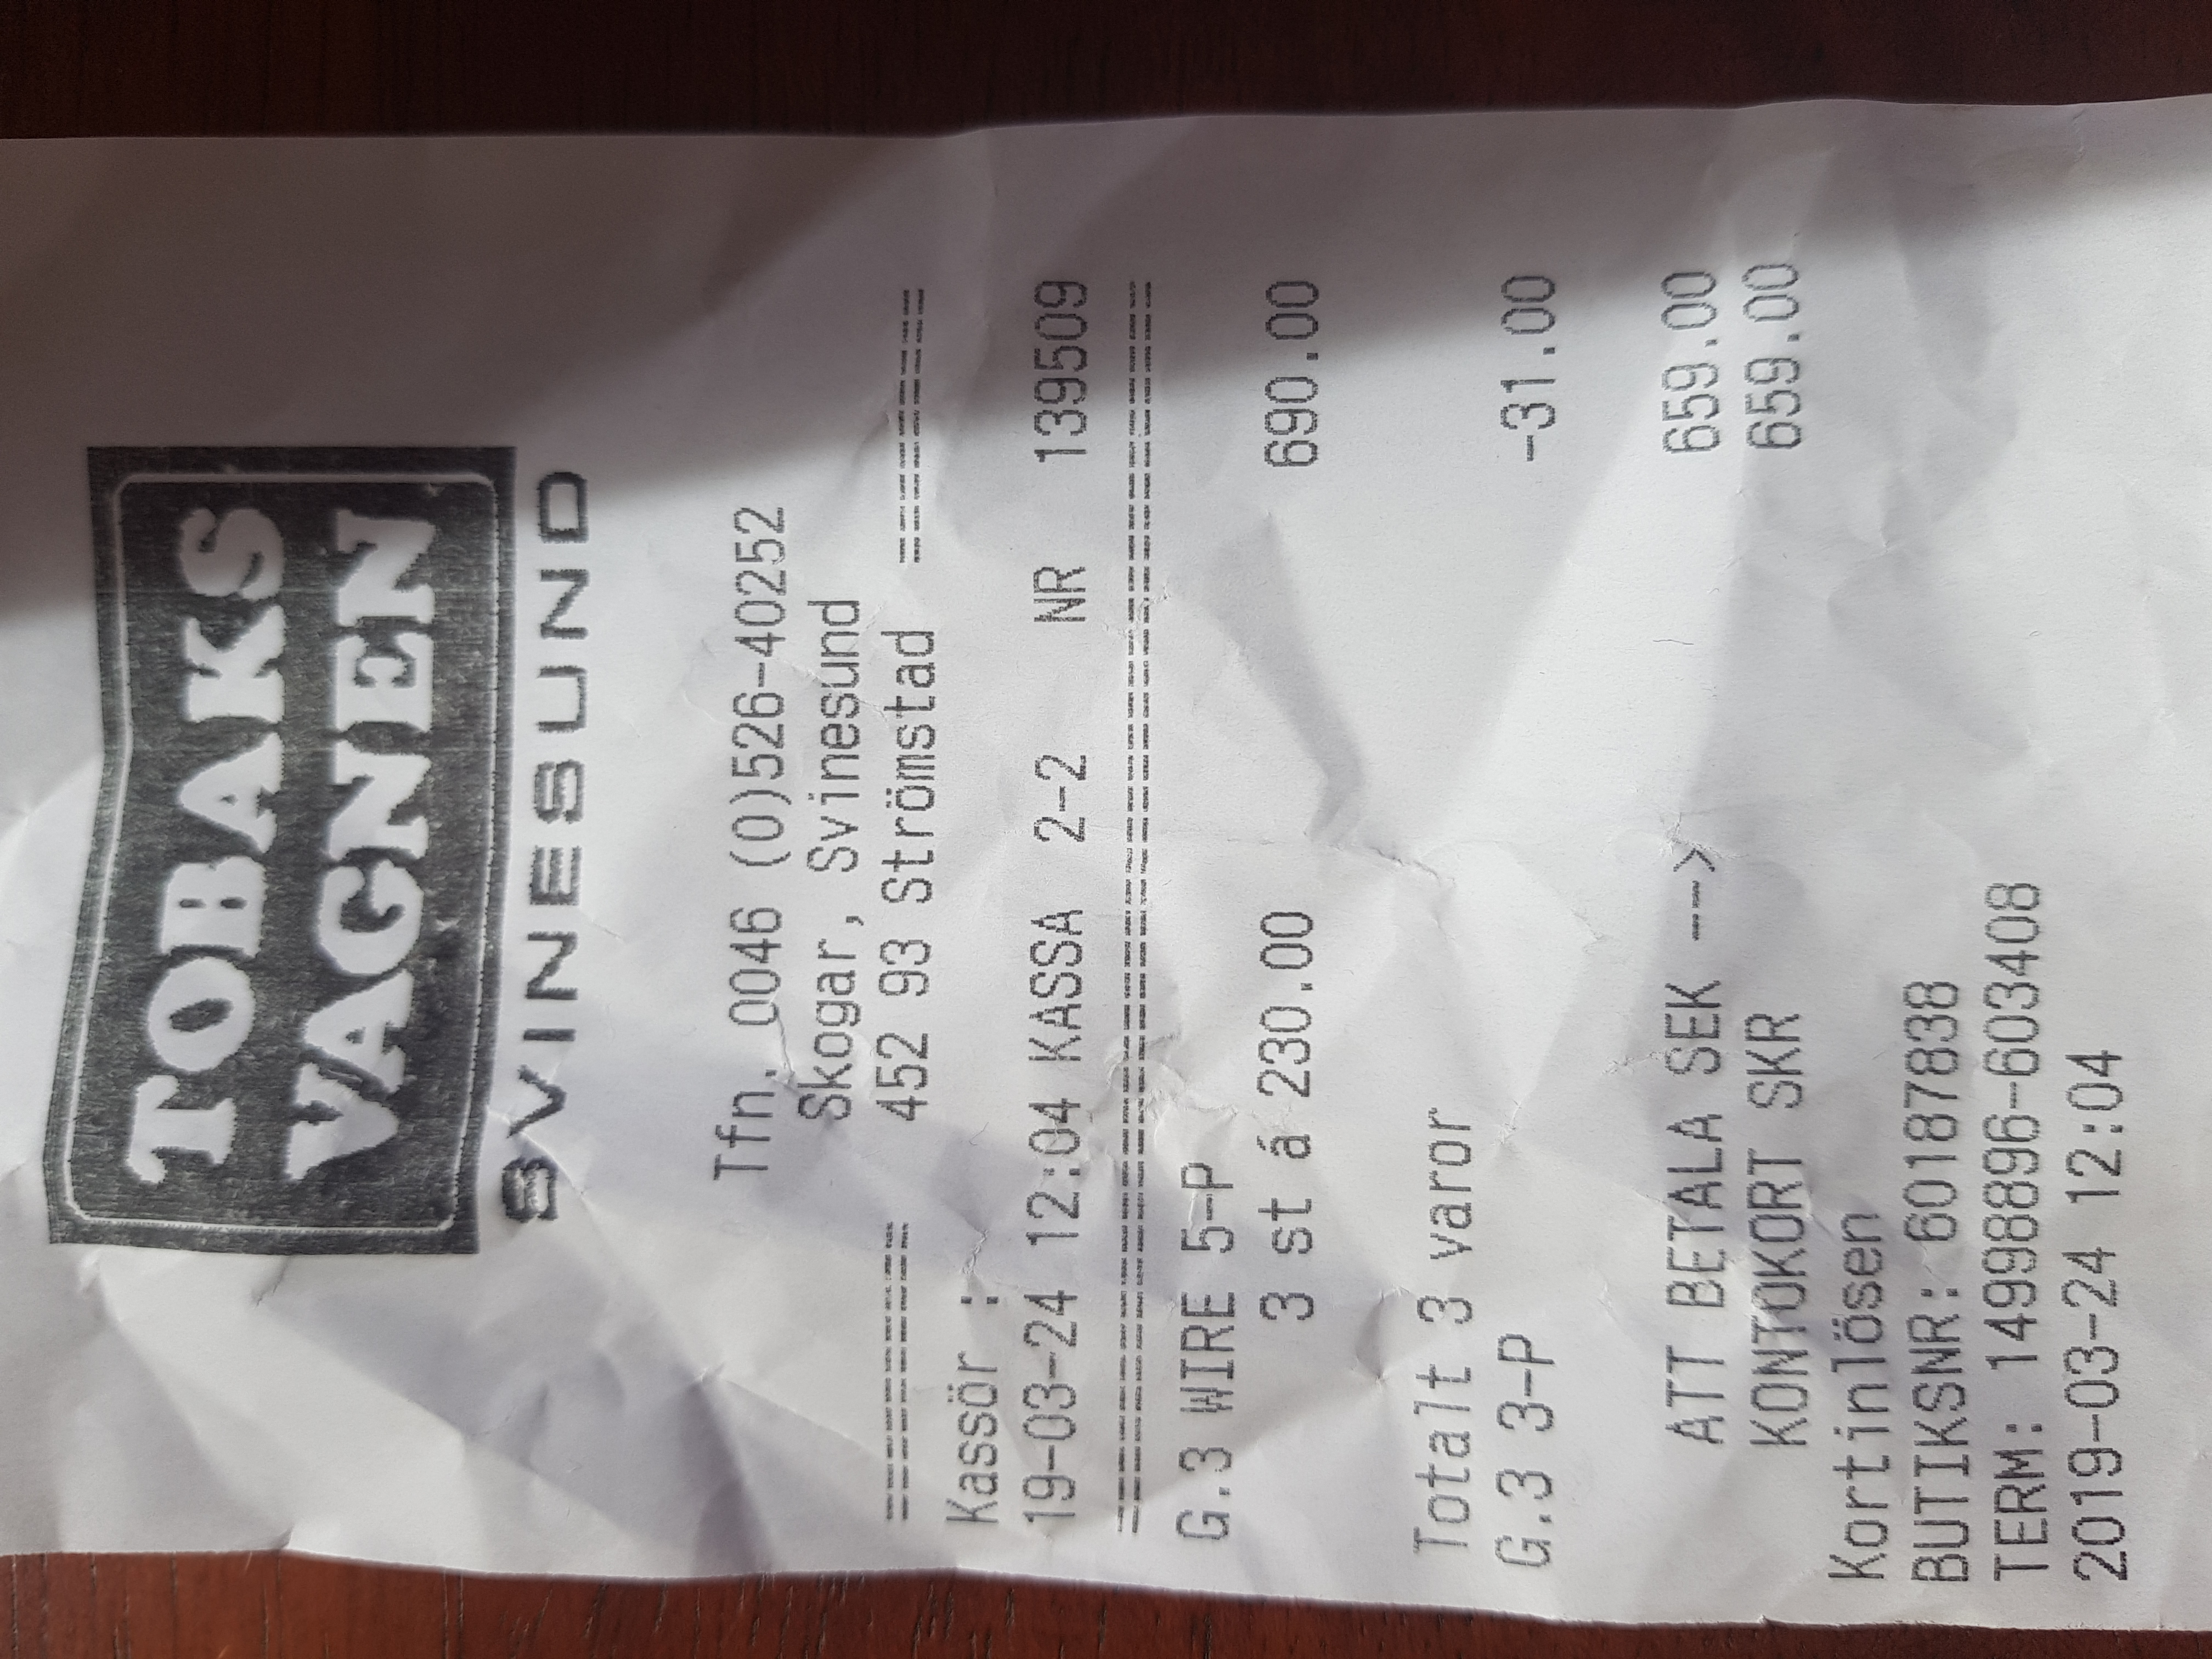
\includegraphics[scale=0.05, angle=-90]{images/kvittering.jpg}
\caption{Eksempel på en kvittering fra en svensk butikk}
\label{fig:kvittering}
\end{figure}

\section{Oppgave}
I dette prosjektet vil vi kun se på teknologien bak analysen av bilde. Det vil ikke inneholde beskrivelse av hva som skjer før og etter denne analysen, som hvordan man får inn bilde som input eller hvordan teksten blir fremvist. Oppgaven blir dermed å få inn et bilde av en kvittering finne ut hva som har blitt kjøpt, prisen, hvor produktet er blitt kjøpt, avslag og eventuelle skatter som har blitt betalt på produktet. Prosjektet kommer til å bruke kodebiblotek og eksisterende teknologier, men egen programkode skal styre retting og behandling av bilde.

\section{Teknologi}
Det finnes mange teknologier innenfor bildebehandling og tekstgjenkjenning. Jeg vil i dette prosjektet fokusere på å velge det som er enklest og implementere og open-source programvare der det er tilgjengelig.
\subsubsection{Tekstegjenkjenning}
Tesseract er et open-source programvare som utfører tekstegjenkjenning. Den kan utfører tekstgjennkjenning på mange typer filformater. Den har også API'er som gjør at det er mulig å bruke det med Python og andre programmeringspråk \footnote{https://www.learnopencv.com/deep-learning-based-text-recognition-ocr-using-tesseract-and-opencv/}. I figur \ref{fig:tesseract_output} ser dere output som blir generert etter å ha skannet bilde i figur \ref{fig:behandlet_kvittering}

\begin{figure}[h]
\centering
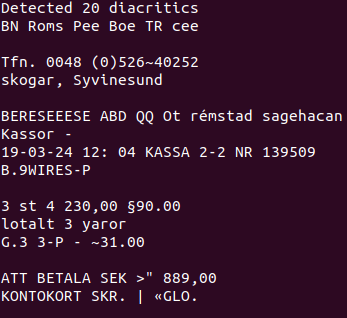
\includegraphics[scale=0.5]{images/output.png}
\caption{Output generert av Tesseract}
\label{fig:tesseract_output}
\end{figure}

\paragraph{Deskewing}
For at bilde skal kunne bli analysert på riktig måte, er vi nødt til skalere, kroppe og rotere bilde. Rotering av bilde kan bli gjort med et konsept som kalles homography. Her kan man bruke referansepunkter på et annet bilde til å rette det. Skalering og kropping er det mulig å programmere selv, eller bruke innebygde funksjoner i scikit-image. \footnote{https://www.learnopencv.com/image-alignment-feature-based-using-opencv-c-python/}
\paragraph{Oppskarpning}
Det kan være utfordrende for tekstgjenkjennings-algoritmer å kjenne igjen tekst. De fleste programmer som kjører tekstgjenkjenning kjører egne filtre for å optimaliser det for tekstgjenkjenning. For å få mer kontroll og øke sjansen for å at gjenkjenningen blir nøyaktig vil jeg bruke min egen optimerer. Den skal kunne gjøre bilde monokromt, fjerne støy, gjøre bilde skarpere og forbedre kontrasten.\footnote{https://docparser.com/blog/improve-ocr-}
\begin{figure}[h!]
\centering
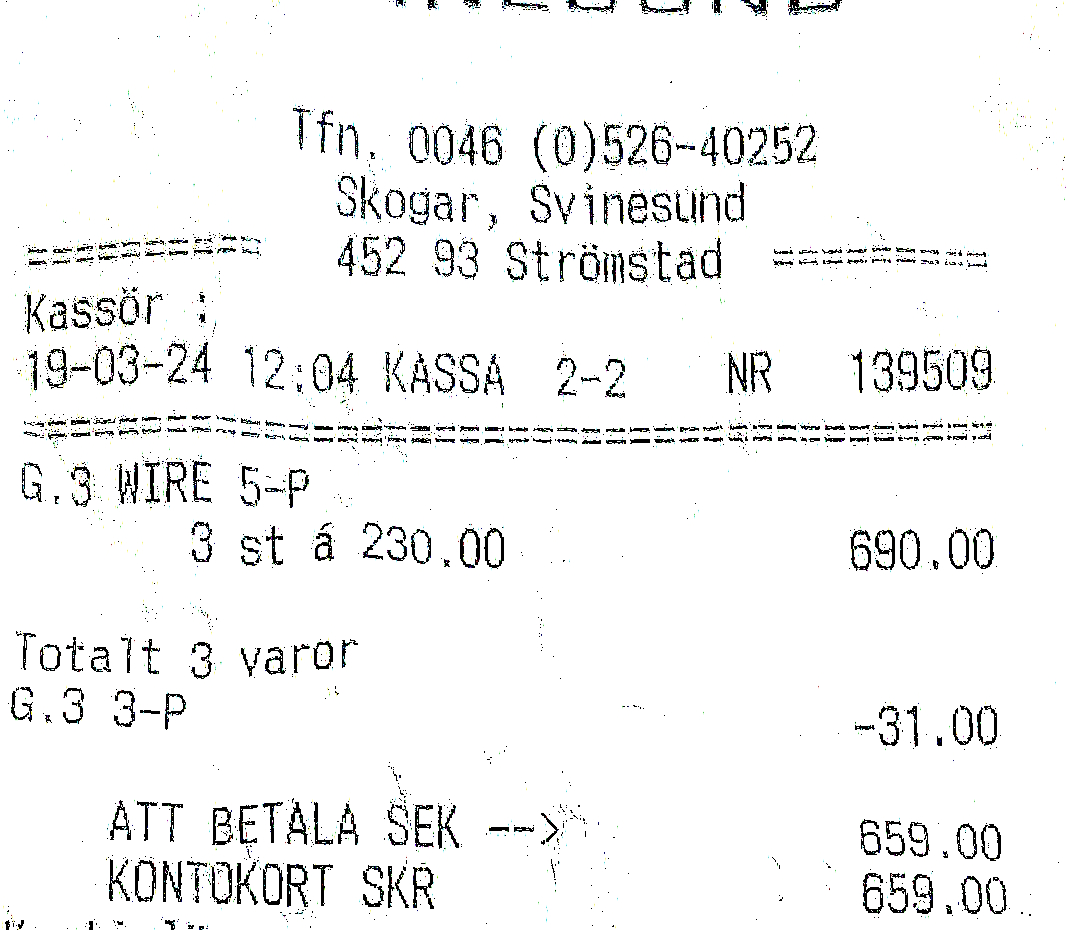
\includegraphics[scale=0.2]{images/test_image_threated.jpg}
\caption{Behandlet versjon av figur \ref{fig:kvittering}}
\label{fig:behandlet_kvittering}
\end{figure}
\footnote{https://docparser.com/blog/improve-ocr-accuracy/}


\section{Gjennomføring}
\subsection{Deskewing}
Et problem med å gjennomføre tekstgjenkjenning på et bilde uten å ha behandlet det først er at man ikke har noen garanti på at bilde har riktig vinkel. Hvis teksten ikke går parallelt med bilde vil resultatet kunne bli dårligere. Som observert i figur \ref{fig:skewed45} er bildet feil orientert. På dette bildet klarer ikke tesseract å gjenkjenne teksten. På bildet som er rikitg orientert får vi følgende resultat som sett i figur \ref{fig:skewed10result}. Dette resultatet er bedre, men fortsatt langt fra treffsikkert.


\begin{figure}[h]
\centering
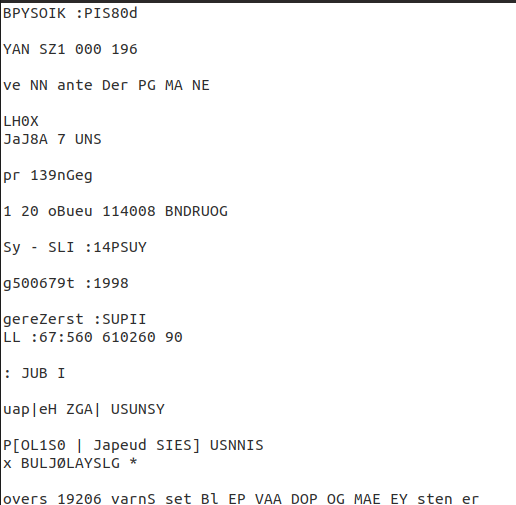
\includegraphics[scale=0.6]{images/skewed10results}
\caption{Resultate av tessearct OCR}
\label{fig:skewed10result}
\end{figure}


\begin{figure}[h]
\centering
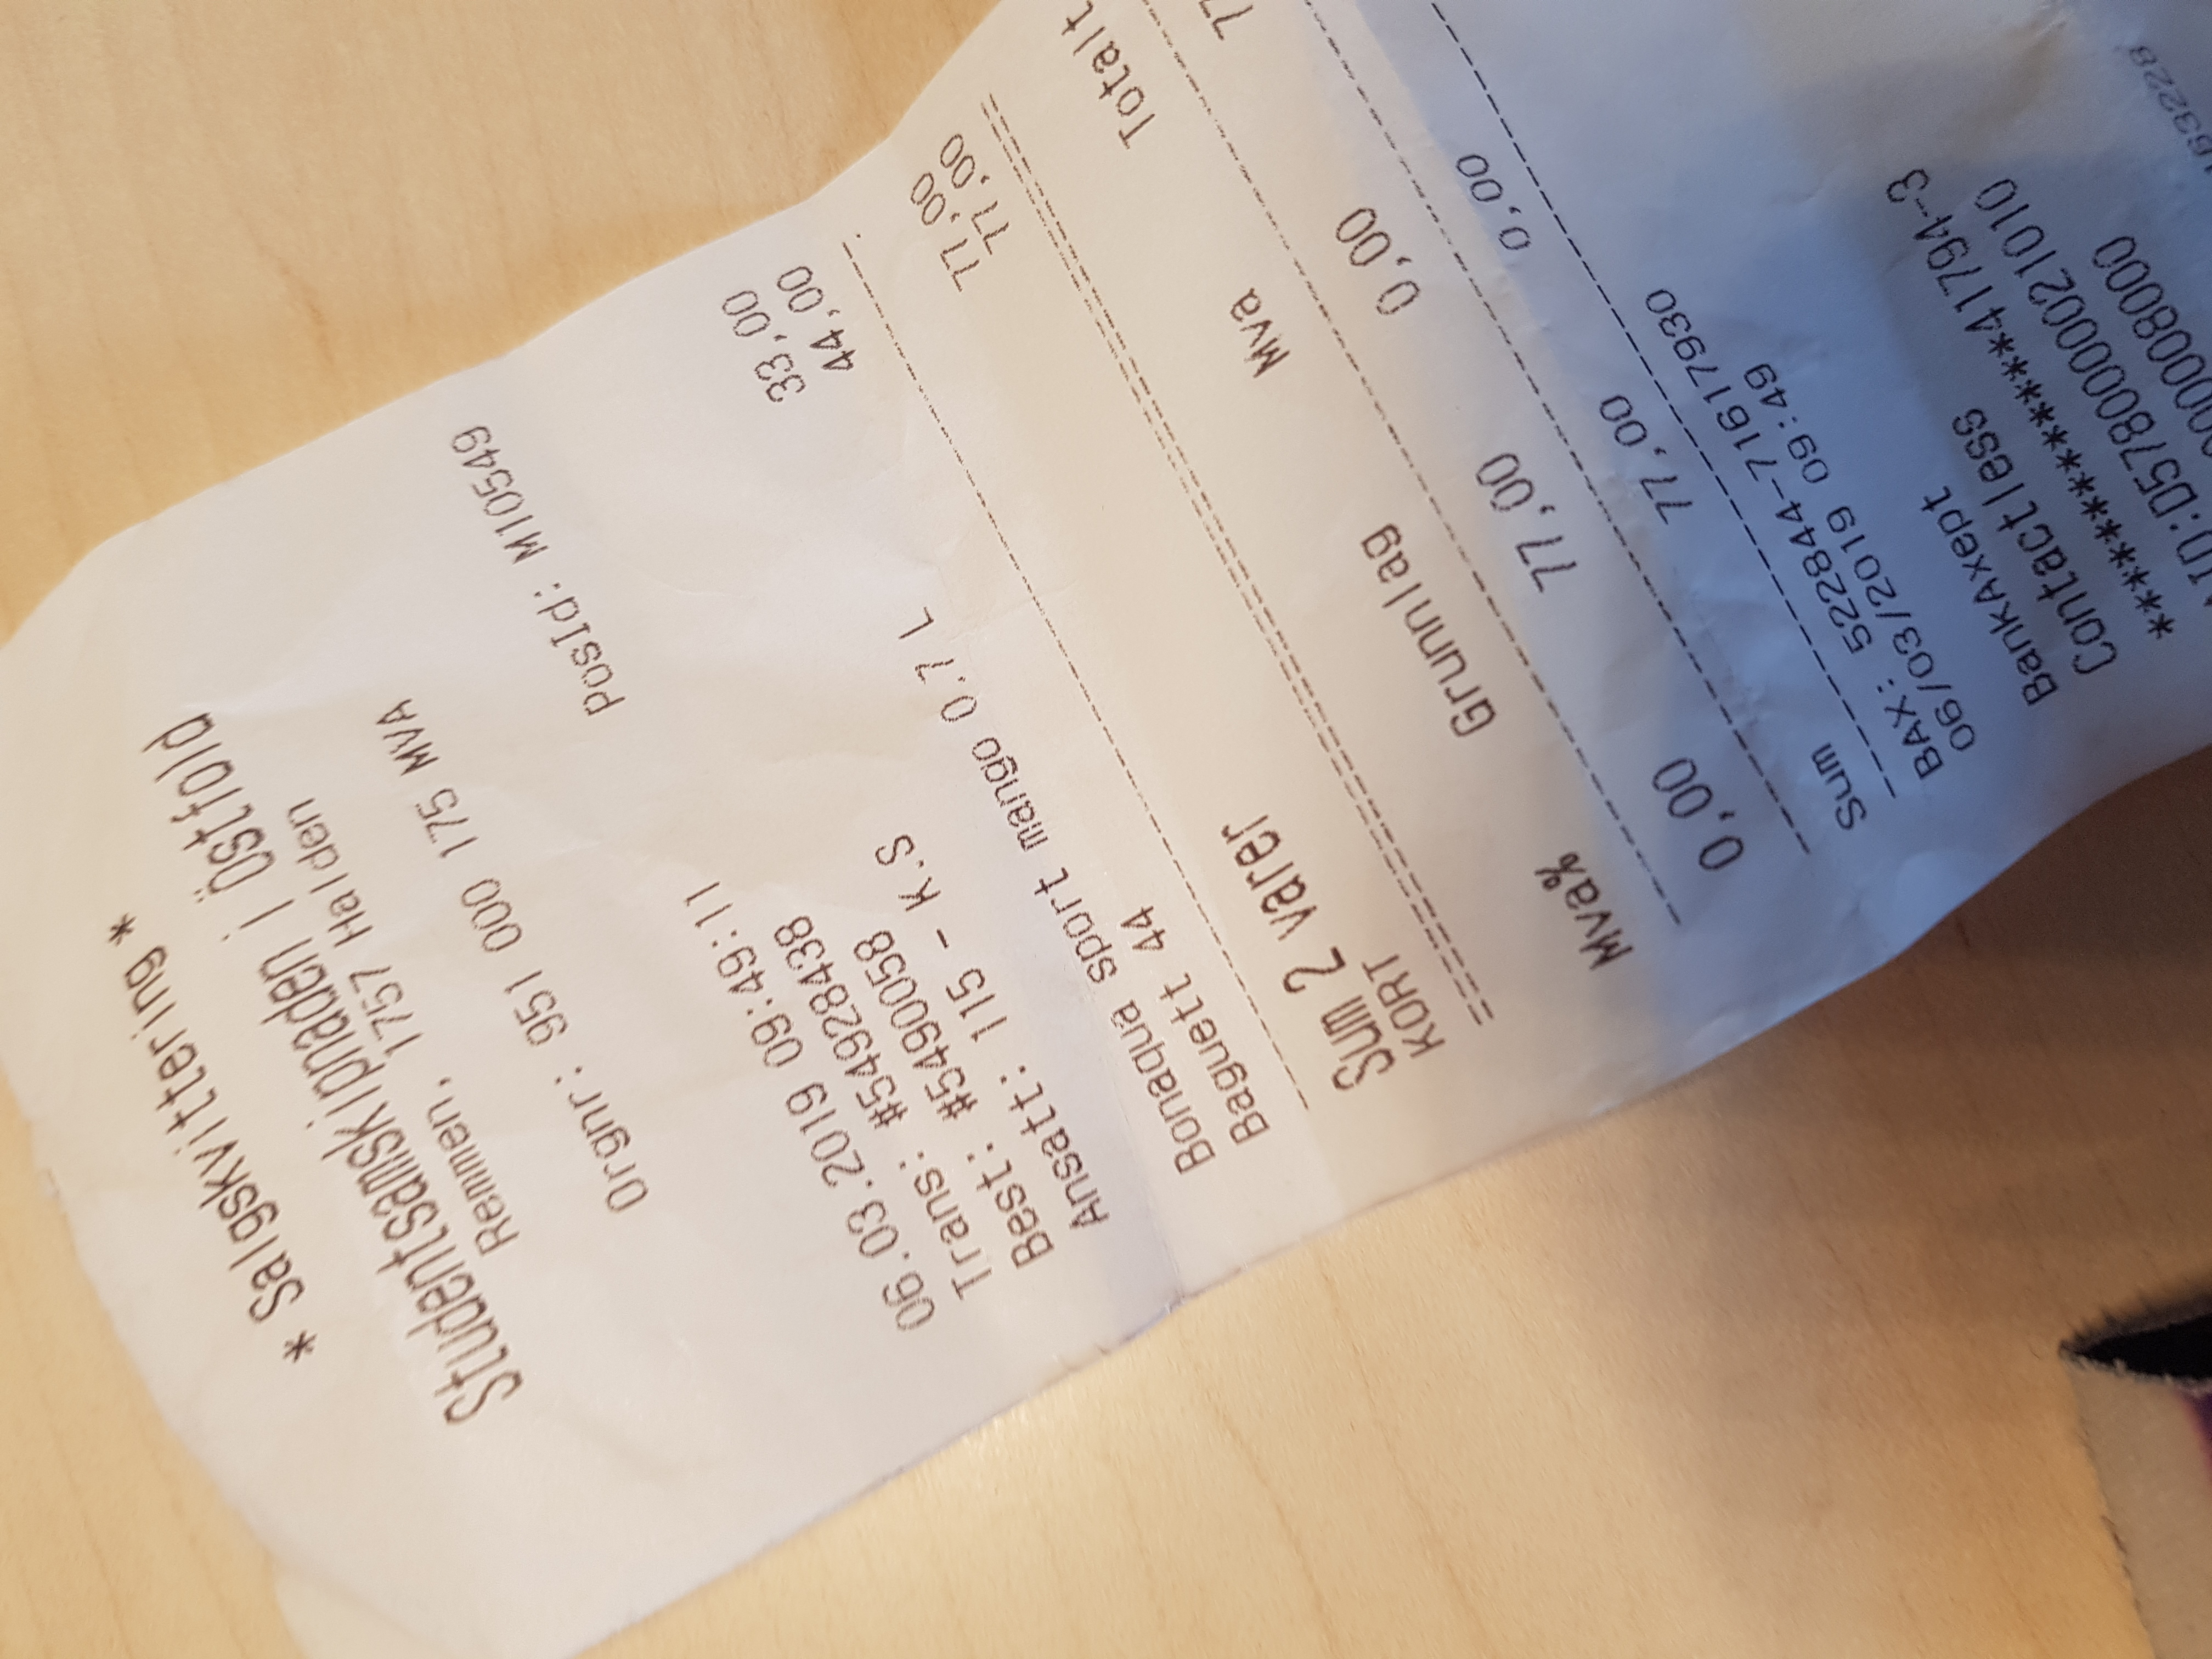
\includegraphics[scale=0.05, angle=270]{images/skewed45}
\caption{Bilde med feil rotering}
\label{fig:skewed45}
\end{figure}

\subsection{Hough}
\paragraph{Teori}
Hough transformasjonen er brukt for å detektere former. Algoritmen har potensiale til å detektere forskjellige typer former, men i denne sammenhengen er den kun nyttig for å detektere linjer \footnote{https://en.wikipedia.org/wiki/Hough\_transform}. Hough transformasjonen baserer seg på at en linje kan bli representert matematisk som $$y = m * x + b$$ eller $$r = x * cos(theta) + y * sin(theta)$$ Problemet med den første formen er at hvis vinkelen blir 90 grader i forhold til den horiontale linjen over bilde vil verdien m, eller stigningen m bli evig stor. Man vil derfor bruke en parameterisert form i polar-koordinater. Variablen r er lengden fra origo til et punkt P på linjen, theta er vinkelen mellom linjen OP og 'initial ray' eller X-aksen på bildet i dette tilfellet.

Med denne parameteriseringen kan vi finne alle linjer som opfyller likningen per punkt på forgrunden av bildet. Da kan vi plotte alle verdiene for r og theta som en graf. Gjør man dette for alle forgrundspikslene i bildet, får vi en graf som viser når linjer krysser hverandre.

Man kan også beregne akkumulator-celler. Her genererer man en matrise hvor kolonenne bestemmer theta og radenen bestemmer r. For hver forgrundspiksel vi har gått igjennom å beregnet hvilke verdier for theta og r som opfyller likingen legger vi til verdien en i legger vi til 1 i akkumulatoren i punkt (r, theta). Hver gang vi legger til 1 betyr dette at vi har funnet en ny piksel som skal bli lagt til på linjen. Dette betyr at vi sitter igjen med hvor mange piksler som ligger på en linje definert av r og theta i denne grafen. Dette kan være nyttig for å finne tydlige linjer i bildet.

\paragraph{Implementasjon}
I et bilde av tekst eller i mitt eksempel et bilde av en kvittering, kan man detektere linjene som blir dannet av teksten.

Jeg valgte å bruke innebygde funksjoner for hough transformasjon i dette prosjektet. Scikit har funksjoner som $hough\_transform$ og $hough\_transform\_peak$ som jeg brukte for selve hough transformasjonen.

Prinsippet er at de mest tydlige linjene fra Hough transformasjonen vil bli valgt ut for seleksjon. I seleksjonen finner jeg hvilke linjer med omtrent samme vinkel som forekommer flest ganger. Håpet er at disse linjene er linjene generert av teksten på kviteringene. Vinkelen til linjene som forekommer flest ganger bestemmer derfor rotasjonen på bildet. Et eksempel på dette kan bli sett i figur \ref{fig:hough-45}. Her har algoritmen funnet flere forekomster av sterke linjer, hvilken vinkel med x-aksen som forekommer flest ganger og deretter rotert bilde med denne vinkelen. I figur \ref{fig:hough-result} ser man listen counter som holder på hvilke vinkler i radianer som forekommer flest ganger. Et problem med denne algoritmen er at den er avhengig av klare linjer. Jeg har kjørt algoritmen på en del bilder og det hender at bildet blir rotert feil vei. Algoritmen tar heller ikke høyde for at bilde kan være opp ned eller rotert over 90 grader.

En løsning på dette ville være å prøve å rotere begge veier for så å sammenlikne tesseract resultatet med en ordbok automatisk for å sjekke hvilken rotasjon som var riktig.



\begin{figure}[h]
\centering
\includegraphics[scale=0.05]{images/hough-rot-45}
\caption{Rotering gjort med Hough transform}
\label{fig:hough-45}
\end{figure}


\begin{figure}[h]
\centering
\includegraphics[scale=0.8]{images/hough-result}
\caption{Utdrag fra deskewing.py}
\label{fig:hough-result}
\end{figure}


\subsection{Otsu tresholding}
\paragraph{Teori}
Otsus metode er en algorimte for tresholding av et bilde. Den baserer seg på intra-class variance. Varians i statistikkens verden er gjennomsnittelig avstand fra gjennomsnittet.
For å finne denne kvadrererman alle verdien som avviker fra gjennomsnittet og legger de sammen. Man deler så pa antall avvik. Intra-class varians er variansen innenfor en klasse.

I Otsus metode finner man histogrammet av input bilde. Optimalt sett vil man se to klasser eller topper innenfor dette histogrammet. Man prøver så å finne en treshold grense k som gjør at intra-class variansen blir så liten som mulig.

Problemet med denne algoritmen er at den er vedldig avhengig av at det histogrammet generert av bilde har to topper. Hvis bilde har mye støy kan dette jevne ut histogrammet og resultatet kan blir dårlig.

\paragraph{Implementasjon}
For å kode denne algoritmen fulgte jeg stegene i kapittel 10.3 i boken Digital Image Processing.
\begin{itemize}
\item Finn histogrammet for input bildet.
\item Regn ut de kumulative distrubisjons funksjonene for begge klassene
\item Finn den kumulative gjennomsnitts funksjonen for den ene klassen
\item Finn den kumulative gjennomsnitts funksjonen for hele histogrammet
\item Finn avstanden mellom klassene (Between class variance)
\item Finn segmenteringen k som gir den lengste avstanden mellom klassene ved å gå gjennom alle k
\end{itemize}

Dette vil gi den beste segmenteringen avhengig av at histogrammet inneholder to klasser.

\paragraph{Resultat}
Algorimten fungerte bra på bilder som ikke inneholdt skygger, eller som var rotert for mye. Skyggene førte til en jevnere overgang av de to klassene i histogrammet. Da jeg fjernet skyggene i bilde og de svarte kantene som er et resultat av rotasjonen av bilde, fungerte algoritmen veldig bra. Jeg fjernet også støy med et gaussisk filter for å få et enda bedre resultat. I figur \ref{fig:otsu-results} ser man input bilde til venstre, det samme bilde segmentert med otsus metode til høyre. Nederst har jeg fjernet kantenen på roteringen og skyggen på nederst på bilde. Segmenteringen blir dermed bedre. På bilde til høyre valgte otsus metode en treshold på 117, på det nederste bilde ble det valgt en treshold på 152.

\begin{figure}[h]
\centering
\includegraphics[scale=0.25]{images/otsu-results}
\caption{Otsu segmentering}
\label{fig:otsu-results}
\end{figure}

\end{document}